\section{Cloth}

\begin{figure}[h!]
\centering
\begin{minipage}[t]{.45\textwidth}
  \centering
  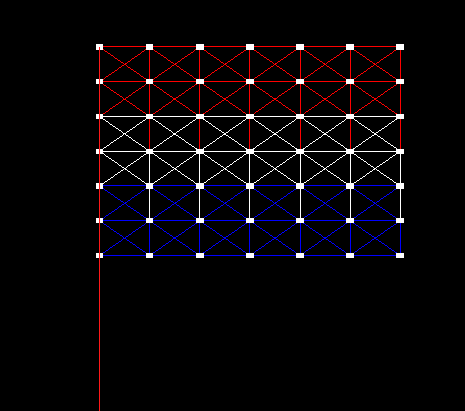
\includegraphics[width=7cm]{img/flag.png}
  \captionof{figure}{Start position of the cloth flag}
  \label{fig:flag}
\end{minipage}\hfill
\begin{minipage}[t]{.45\textwidth}
  \centering
  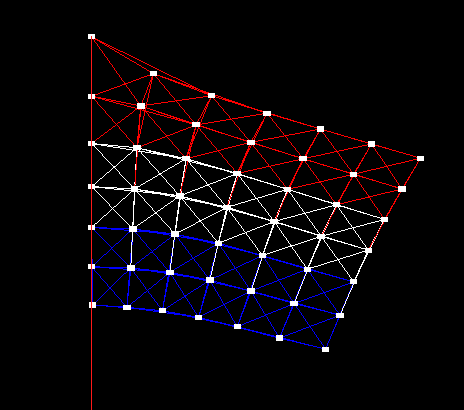
\includegraphics[width=7cm]{img/flag2.png}
  \captionof{figure}{Position after some iterations}
  \label{fig:flag2}
\end{minipage}
\end{figure}

\noindent The structure of the cloth contains of multiple spring forces.
First a grid of spring forces is created.
Then in each cell of the grid two cross springs are added, creating a cross in each cell.
Finally a spring of twice the length is added to each point of the grid, connecting two cells.
This structure will result in quite a realistic piece of cloth.
In figure ~\ref{fig:flag} and ~\ref{fig:flag2} a Dutch flag is modeled, the pole is a fixed object with a particle constrained in the left top using a Fixed constraint. Also all left particles are constraint using a vertical line constraint.